\section{Context Free Grammar Stats}
\label{cfgstats}
\subsection{Introduction}
Fuzzing with context free grammars is done by making choices. Specifically, a
rule needs to be chosen at each non-terminal, each of which includes additional
terminal and/or non-terminal symbols. Eventually, after making many choices, a
point is reached in where there is no other non-terminal left to choose rules
from and one is left with a string of terminal symbols.

The ``quality'' of the generated output depends upon the choices
which are made. Therefore, it is critical to have some sort of way of making
``good'' choices: some way other than simply choosing a random rule from a
non-terminal. This is where statistics come in.

If Fuzzbuzz is able to take in various tables of statistics then it will
inherently be able to make informed choices. For example, a basic statistics
table might include production probabilities. That is to say, given some
non-terminal and its set of rules, what are the probabilities for each rule?
Given the following simple grammar, the table would provide $\mathbb{P}[B]$,
$\mathbb{P}[C]$, and $\mathbb{P}[D]$ where $\mathbb{P}[B] + \mathbb{P}[C] +
\mathbb{P}[D] = 1$.

\begin{align*}
A &\rightarrow B \\
&\rightarrow C \\
&\rightarrow D \\
\end{align*}

\noindent
This is certainly much better than making random choices, but it is still
rather basic. We now present a literature review of picking rules given a CFG.

\subsection{Literature Review}

Maurer\cite{Maurer1990} gives a wide range of ideas for choosing rules. In his
paper, he describes a simple calculator grammar and then focuses on various
ways he could use the grammar to test his calculator program. He gives various
ideas for picking rules, though he does not go in depth as to whether following
them produces better results. He mentions how one possibility is to avoid
choosing the same rule twice, or how perhaps rules should be chosen in a
particular order. Maurer, however, focuses a lot on user customization,
something which we do not. For example, Maurer suggests altering the
probabilities manually (which he refers to as weights). He reasons that by
doing so, one can generate tests which focus more in a particular area that is
believed to have bugs.

Maurer also suggests keeping track of the number of bugs encountered when a
particular rule is chosen, and then auto adjusting the probabilities to favor
those rules which detect the most bugs. We found this to be an interesting
approach.

Sirer and Bershad\cite{Bershad1999} describe their experience with using
production grammars in order to test software. Their paper does not exactly
propose ways of using statistics to pick rules, though it does suggest other
criteria you can use in order to come to a decision. The authors were working
primarily with the Java programing language, and as such some of their ideas
cater to Java specifics, though are nevertheless interesting enough to be
mentioned in this paper.

One approach which Sirer and Bershad discussed was imposing a limit on how many
times specific grammar rules can be exercised. This is especially useful in
languages like Java that have structural limits such as code length per
method. The authors describe another way in which this can turn out to be
useful: if one wants to ensure that the program doesn't ``terminate early''
(i.e. that it is of a minimum length) is to, for example, set a limit on your
start symbol to 5000 and then a probability of zero on the production $S
\rightarrow \lambda$. This will ``force'' a stop rather than ``naturally''
stopping.

In addition to using production limits, Sirer and Bershad also mention how
probabilities are of good use and emphasize the usefulness of separating
probabilities from the grammar. This is effectively what we do by having
Fuzzbuzz take a statistics table as a parameter which is distinct from the
actual grammar file.

Finally, Sirer and Bershad mention how in order to simplify future test
selection and analysis, for each test case produced they create what they call
a ``summary file'' which lists the name of the grammar rules that have rise to
the test case.

Though we did not find a paper which described conditional probabilities, we
did implement a routine in Gramstats which outputs conditional probabilities.
The conditional probabilities table describes what the probability of choosing a
specific rule is given what the previous N non-terminals were that led to our
current non-terminal. Our hypothesis was that knowing this information would
allow us to make better choices. For example, consider the following grammar:

\begin{align*}
S &\rightarrow A \\
&\rightarrow A B \\
A &\rightarrow B C \\
&\rightarrow C \\
B &\rightarrow r C \\
&\rightarrow r \\
C &\rightarrow s B \\
&\rightarrow q \\
\end{align*}

\noindent
where uppercase letters are non-terminal symbols and lowercase letters are
terminal symbols.


In this example, one could see how the probabilities for the rules $B
\rightarrow rC$ and $B \rightarrow r$ might differ depending on what the
previous non-terminals were. For example, perhaps there is a much higher
probability of choosing $B \rightarrow r$ compared to $B \rightarrow rC$ if the
previous two non-terminals were $S$ and $A$ respectively. On the other hand, if
we arrive at $B$ though $A$ and $C$ respectively, then perhaps there is a
higher probability of choosing $B \rightarrow rC$ over $B \rightarrow r$.

Conditional probabilities allow us to keep more context than pure production
probabilities alone.

It is worth noting that the more you remember (i.e. the higher N is), the more
specific you become and thus the harder it is for Fuzzbuzz to actually be in
that state when generating. For example, taking an arbitrary grammar, if N=2,
then your ``memory`` could possibly be $F, R$ whereas if N=5, it could possibly
be $F, R, G, T, Q$. You can see how it is ``easier`` to land in a state where
your previous non-terminals are $F, R$ than $F, R, G, T, Q$. If while in some
iteration generating output the previous non-terminals are $F, R, G, X, Q$ then
$F, R$ passes but $F, R, G, T, Q$ does not.

\subsection{Results}

First, it should be noted that the CFGStats engine does not produce
semantically correct output. For example, a Fuzzbuzz run using a
grammar which described calculator input produced the following:

\begin{verbatim}
( 2.74432441811 + 1.86534745663 - < 0.424813324932 , 6.79695572322 ^
0.285722493924 > )
\end{verbatim}

This is trying to subtract a vector from a natural number. This is not a
mathematically legal operation, and thus should not ever be outputted from a
fuzzer that produces semantically correct results. However,

There are two variants of the statistics tables: pure production probabilities
and conditional probabilities. Each of these can be passed to Fuzzbuzz as
arguments using the CFGStats engine. The hypothesis is that production
probabilities do not capture the probability distribution as well as
conditional probabilities are able to.

We attempt to show this result by using Fuzzbuzz's sister program, Gramstats.
Gramstats takes in a corpus of example ASTs conforming to some grammar and
outputs statistics based on that corpus. We first used Gramstats to produce
statistics based on a corpus of 190 human generated examples, first using the
production probabilities table and then using the conditional probabilities
table.

Then, using each of these statistics, Fuzzbuzz is able to generate output which
is then fed into Fuzzbuzz again, but using the AST Generation engine. This was
done 400 times in order to generate a different corpus. Then these 400 ASTs are
again parsed by Gramstats to get statistics on them.

This allows us to compare the statistics for natural examples with the
statistics for artificially generated examples, which in turn used the natural
statistics as input. Ideally, the statistics should match.


\begin{figure*}
    \begin{center}

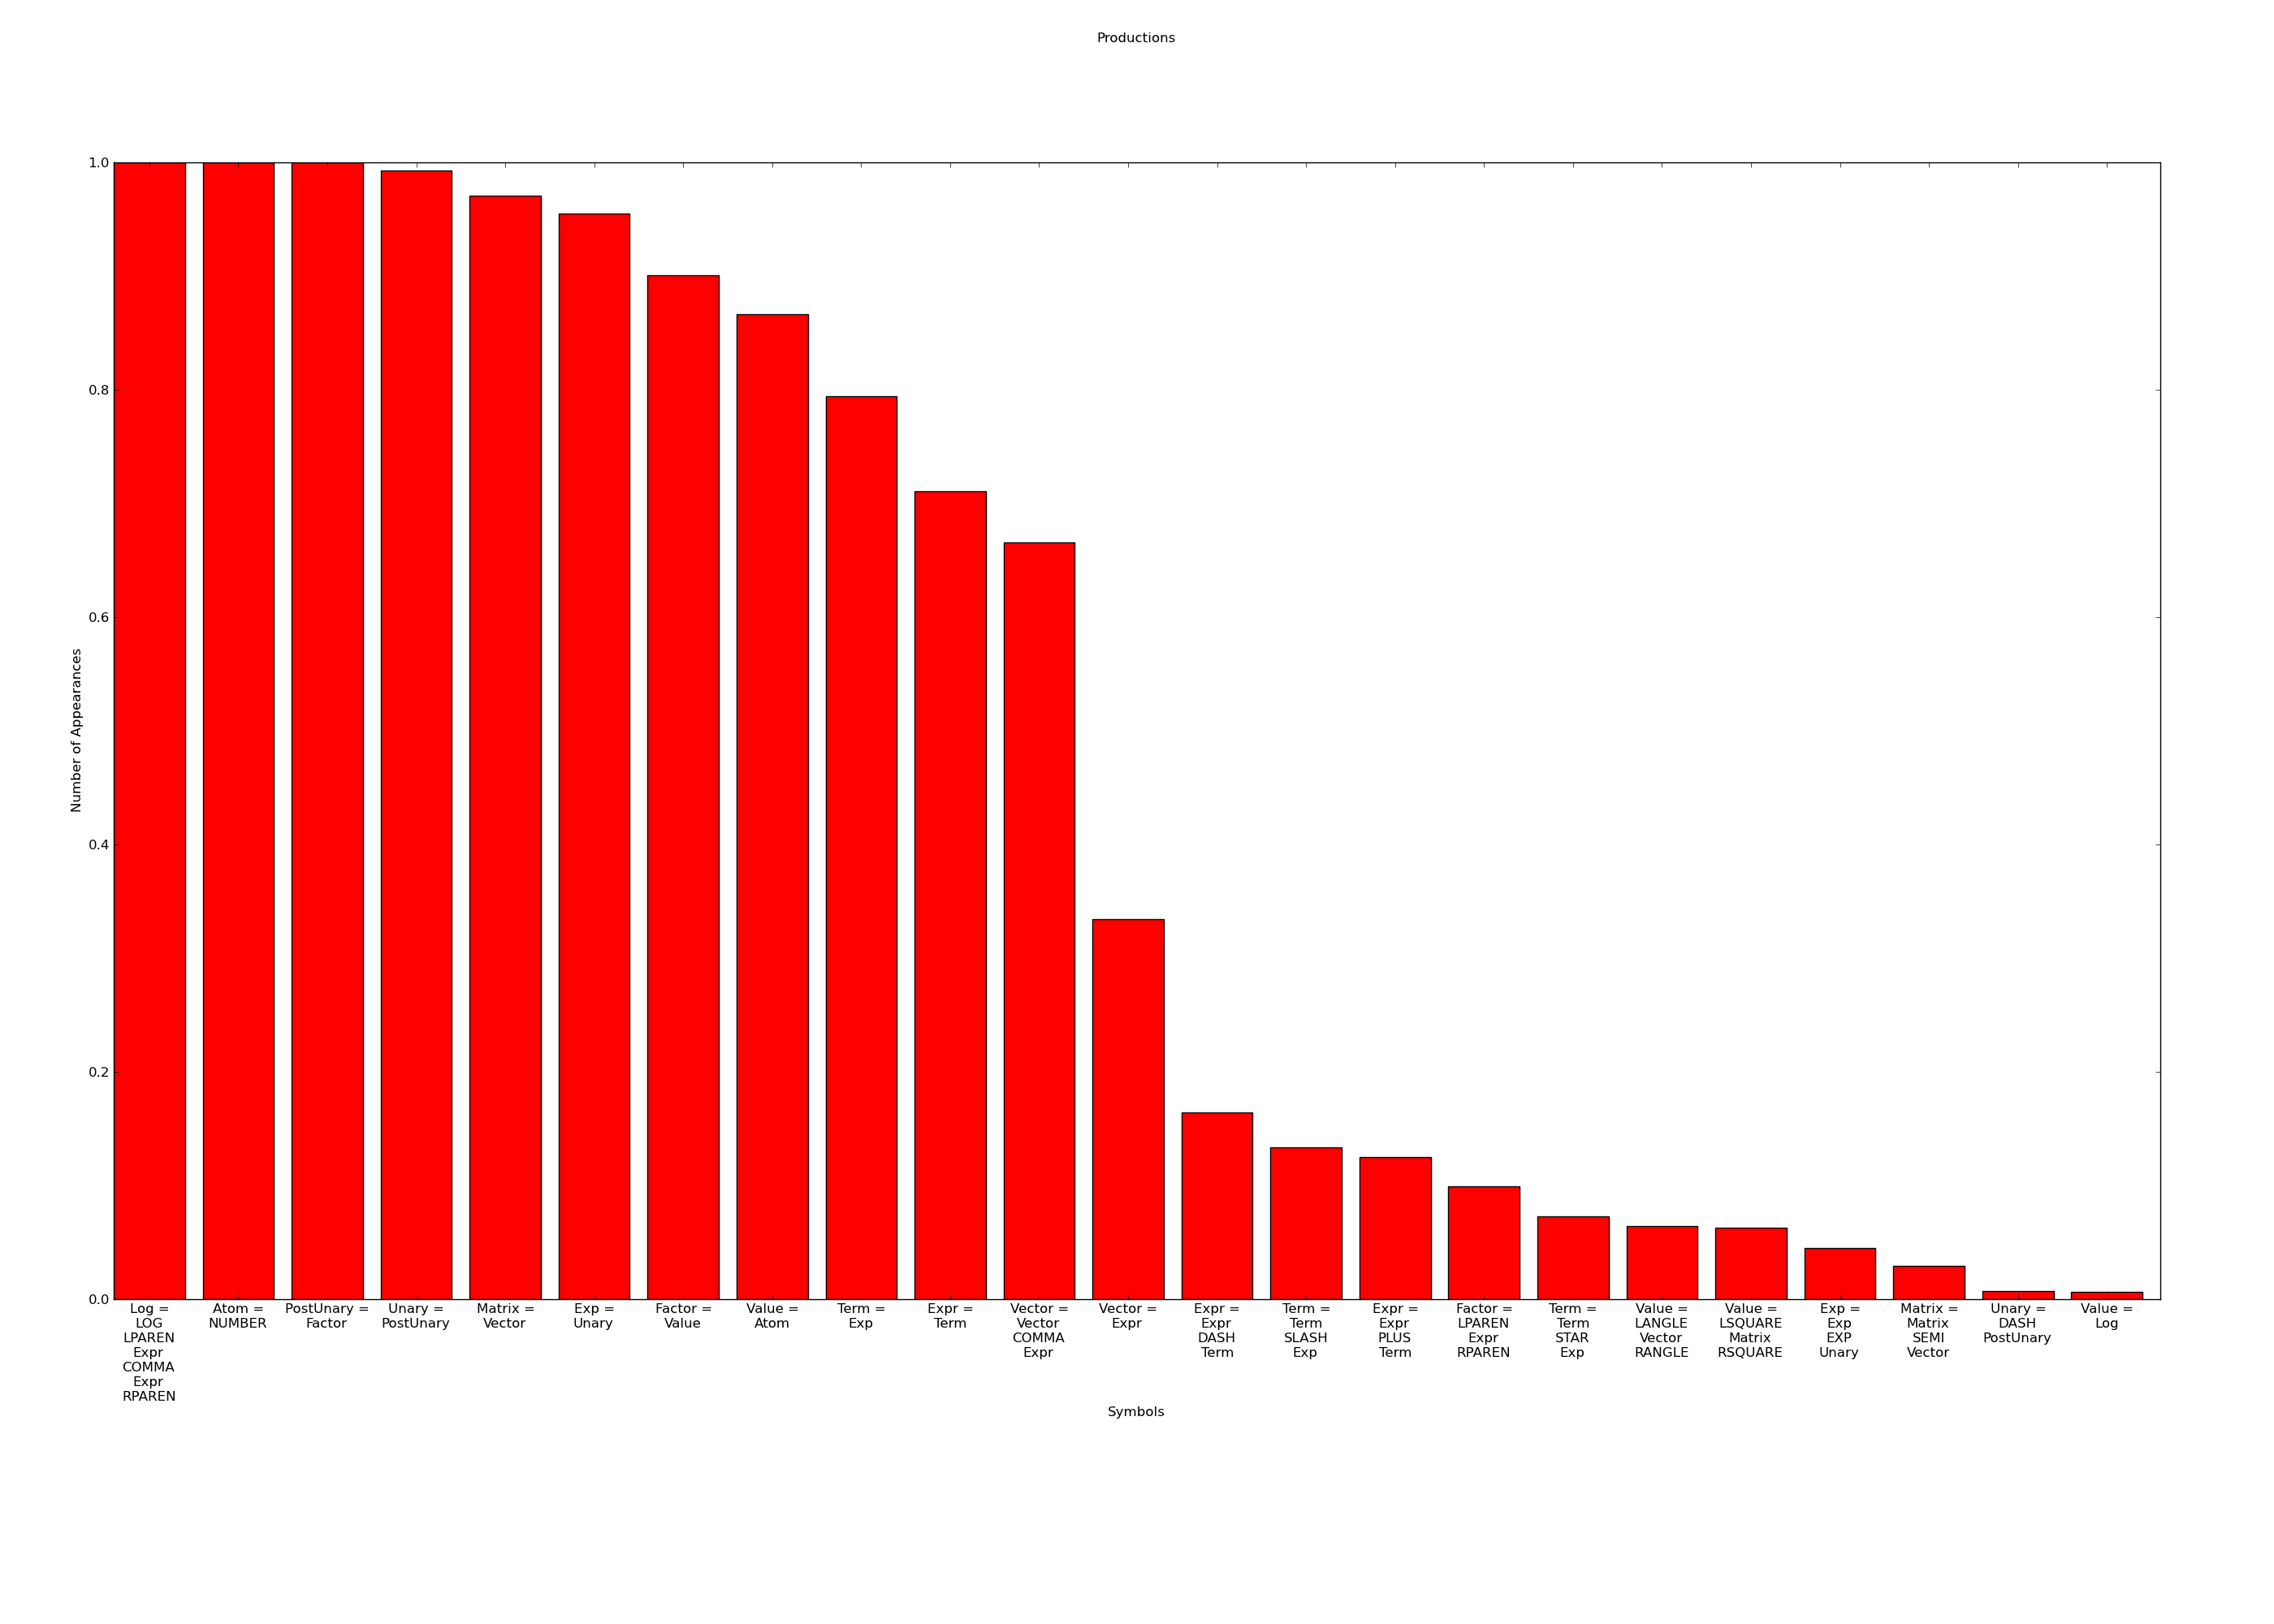
\includegraphics[scale=0.23]{figs/human/production_probability_histogram.png}
    \end{center}
        \caption{Production probability histogram when using a human corpus of
190 example inputs for a calculator program.}
    \label{times}
\end{figure*}

\begin{figure*}
    \begin{center}

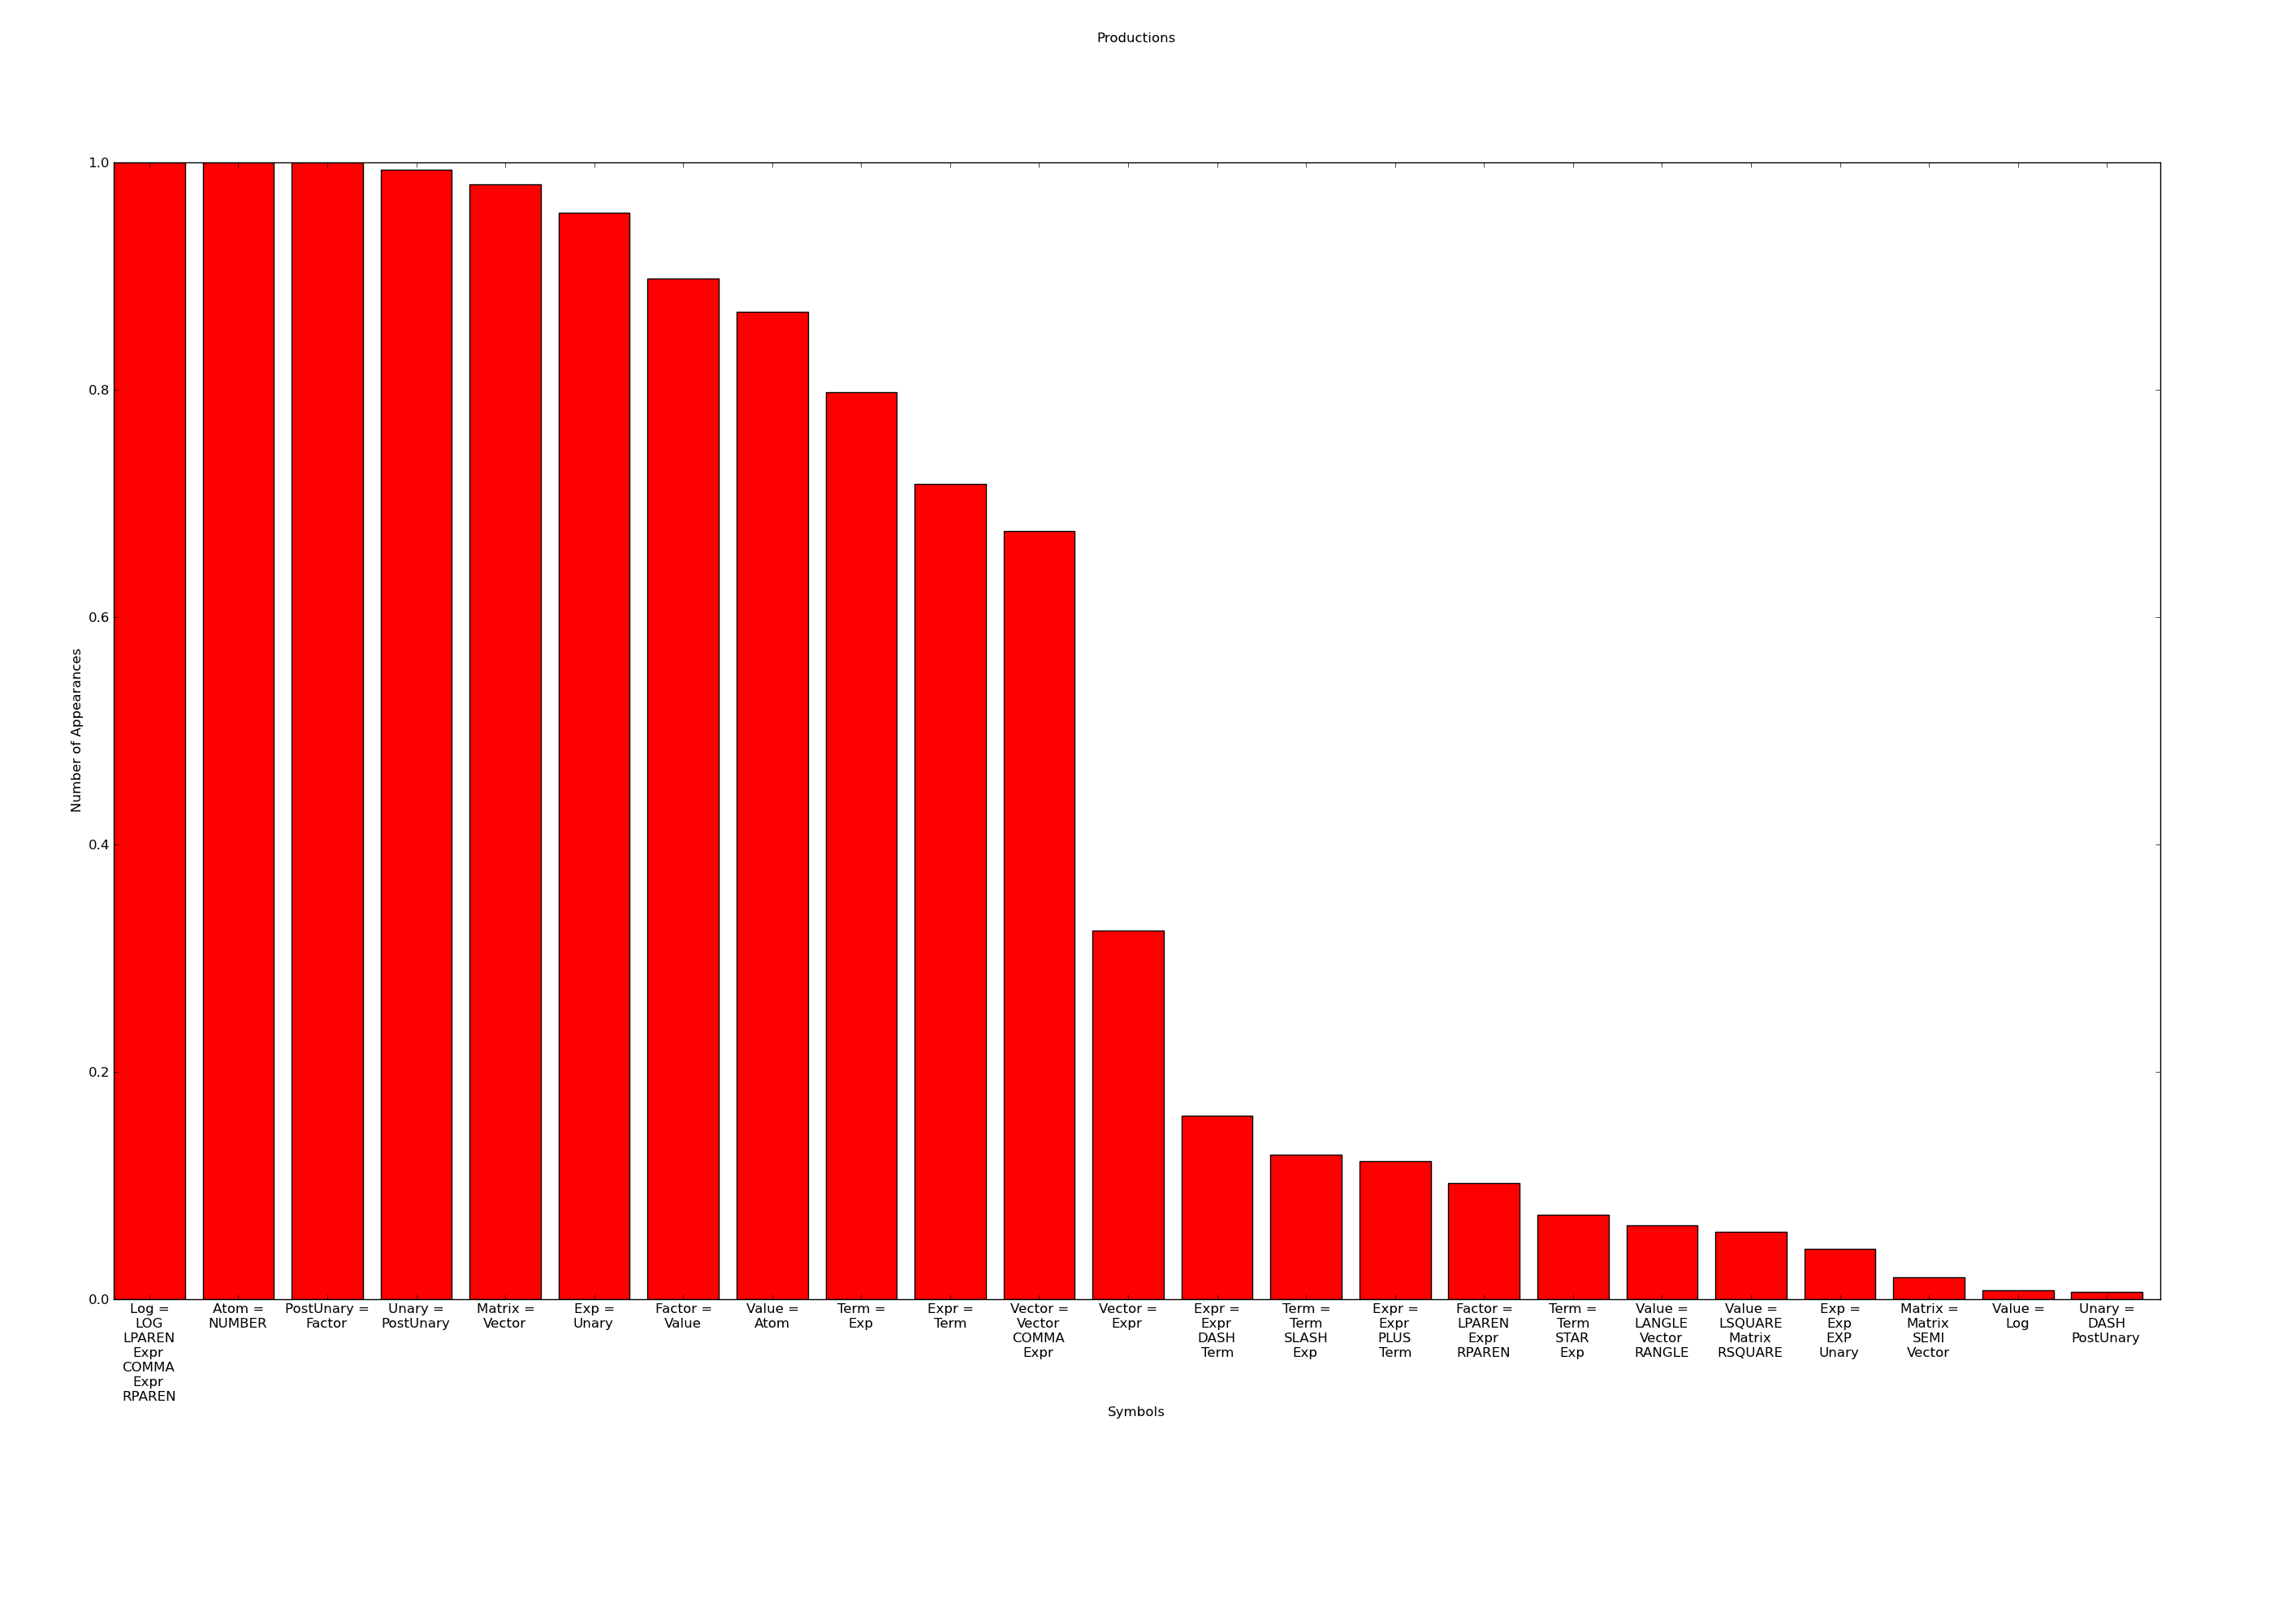
\includegraphics[scale=0.23]{figs/gen/pp/production_probability_histogram.png}
    \end{center}
        \caption{Production probability histogram when using production
probabilities
to generate an artificial corpus of 400 example inputs for a calculator
program.}
    \label{times}
\end{figure*}

\begin{figure*}
    \begin{center}

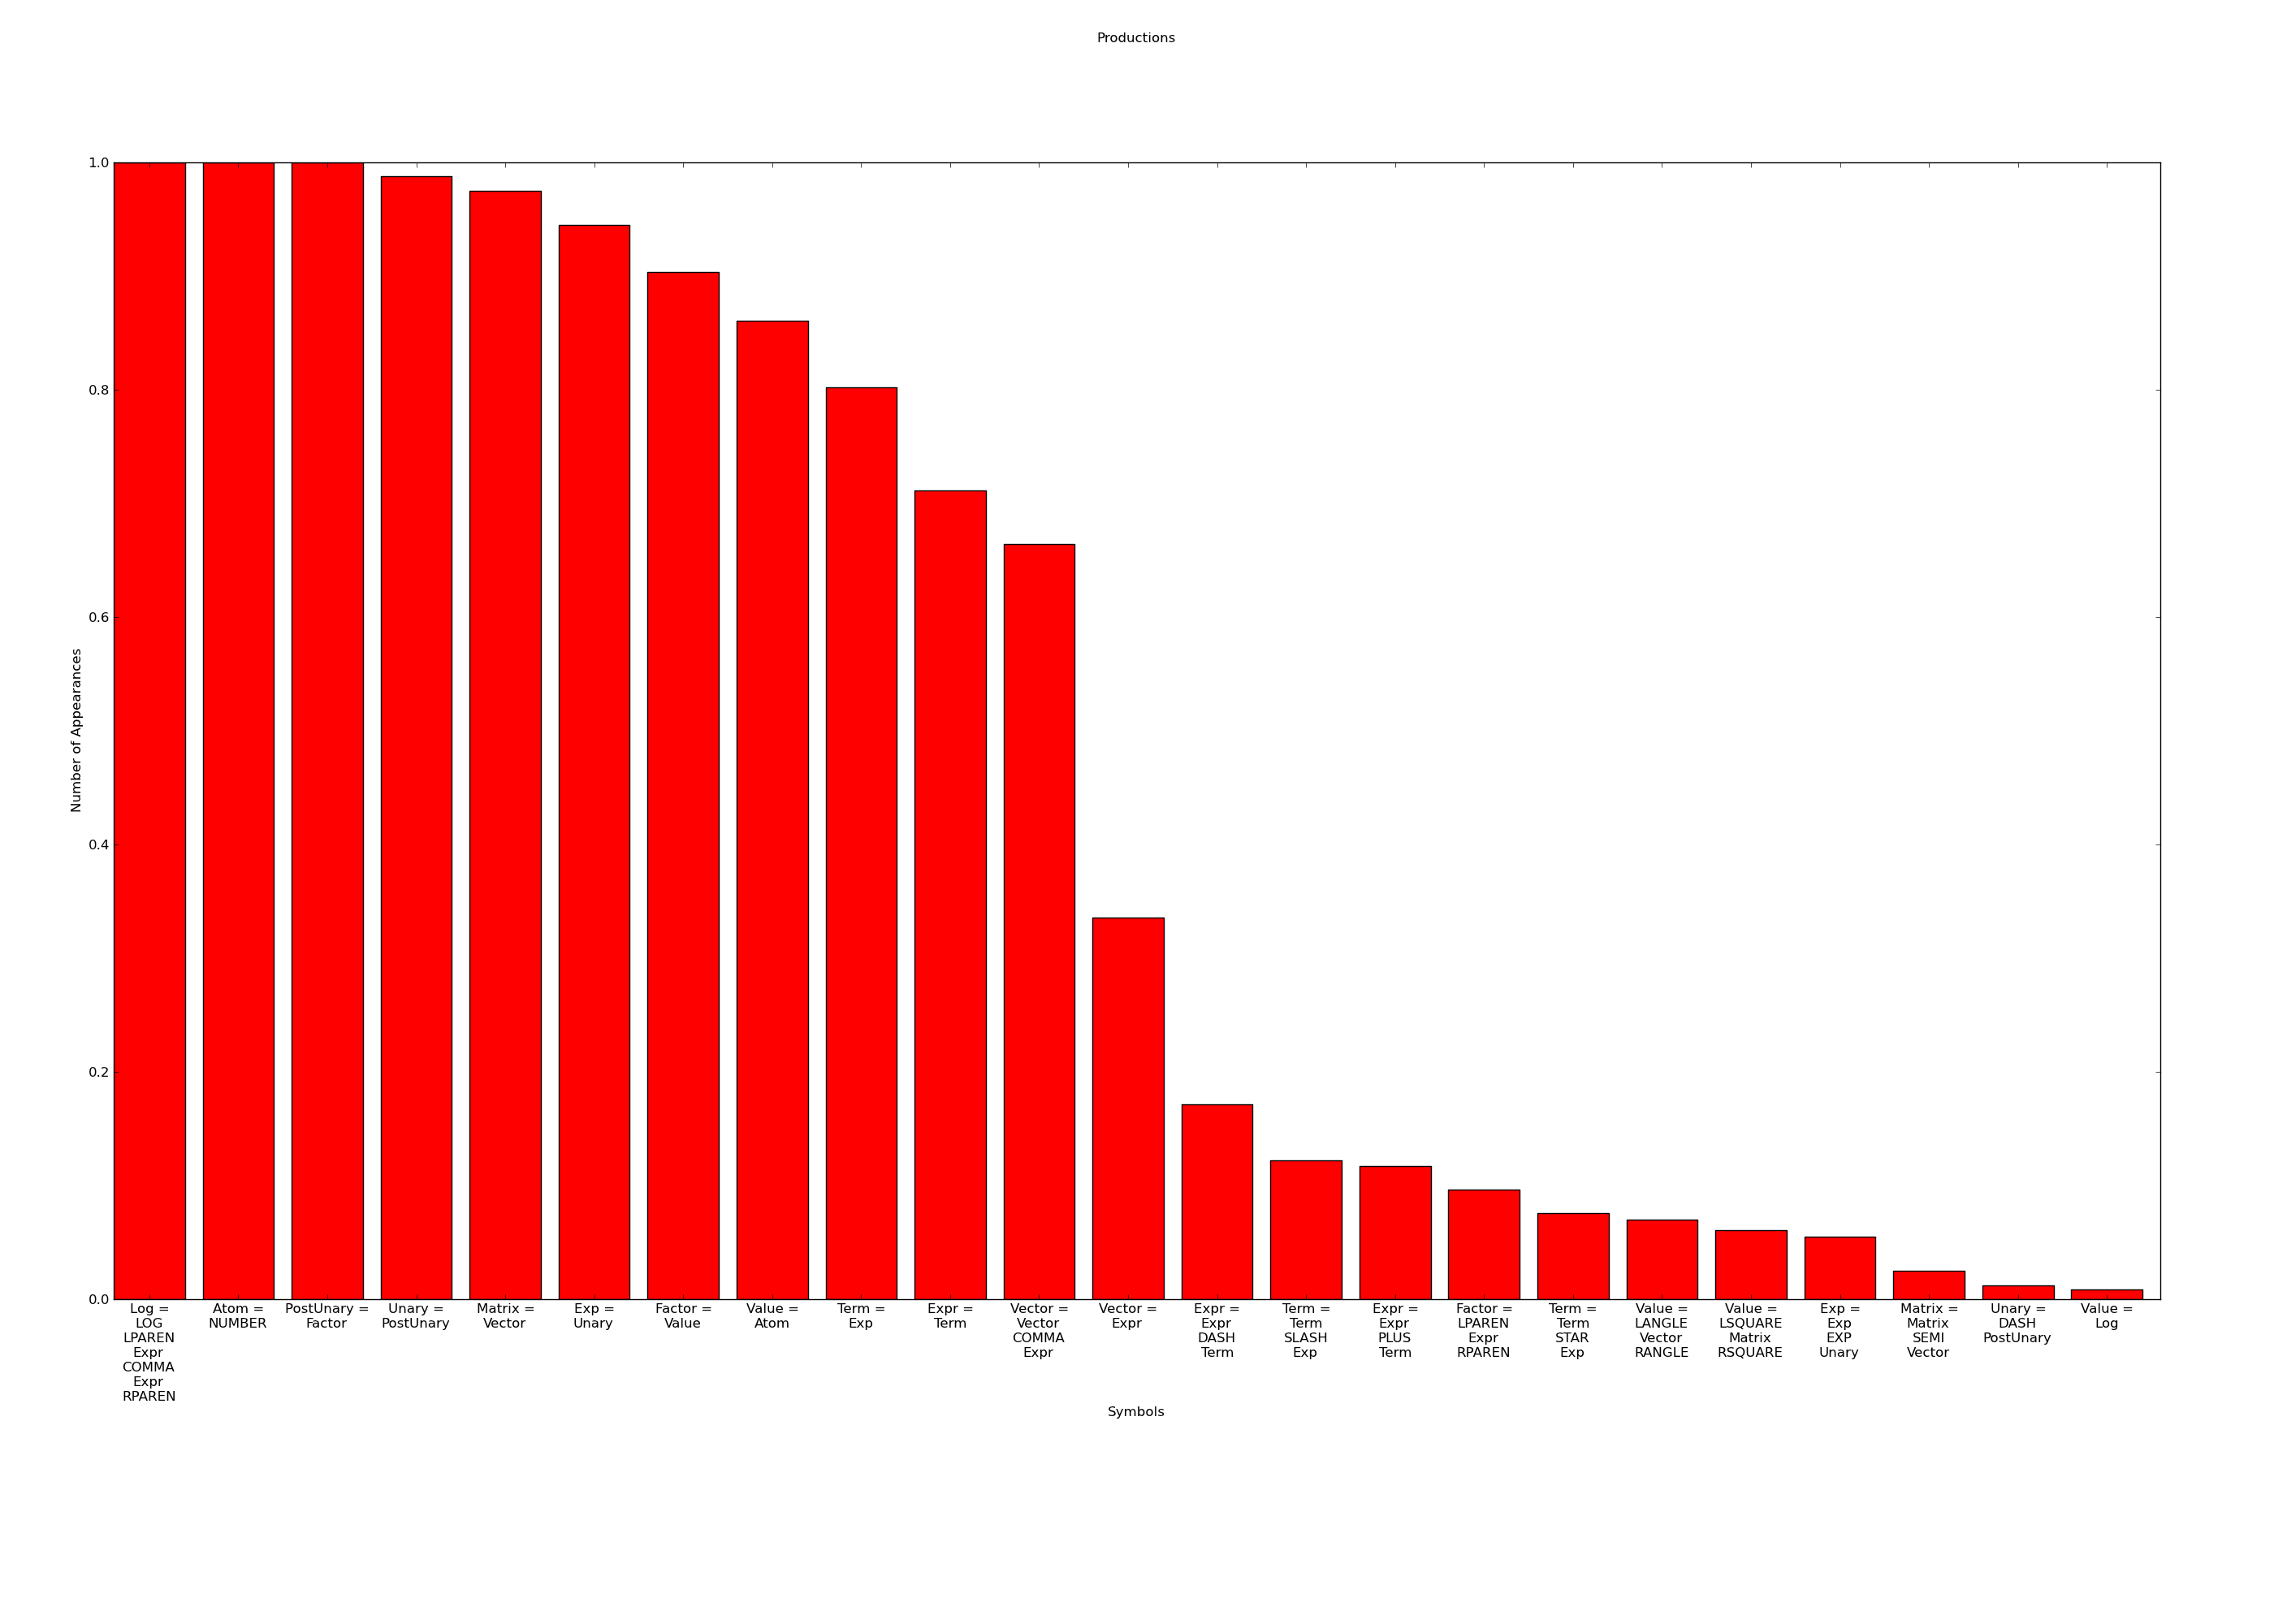
\includegraphics[scale=0.23]{figs/gen/production_probability_histogram.png}
    \end{center}
        \caption{Production probability histogram when using conditional
probabilities to generate an artificial corpus of 400 example inputs for a
calculator program.}
    \label{times}
\end{figure*}


There is no immediate difference between these three graphs. Upon closer
inspection however, differences between the example input sets are evident. Let
us examine the statistics for the $Exp => Exp:EXP:Unary$ rule from the
calculator grammar.

The human corpus produced the following 3 conditional probabilities: \\

\noindent
\begin{verbatim}
2, Exp => Exp:EXP:Unary, Expr, Term, 0.0745580322829
2, Exp => Exp:EXP:Unary, Term, Exp, 0.01398603413986
2, Exp => Exp:EXP:Unary, Term, Term, 0.00726744186047
\end{verbatim}


The artificial corpus generated using production probabilities produced the
following 13 conditional probabilities: \\

\noindent
\begin{verbatim}
2, Exp => Exp:EXP:Unary, Expr, Expr, 0.2
2, Exp => Exp:EXP:Unary, Expr, Term, 0.0460969044415
2, Exp => Exp:EXP:Unary, Exp, Term, 0.0289855072464
2, Exp => Exp:EXP:Unary, Factor, Expr, 0.037037037037
2, Exp => Exp:EXP:Unary, Factor, Term, 0.0485436893204
2, Exp => Exp:EXP:Unary, Factor, Value, 0.103448275862
2, Exp => Exp:EXP:Unary, PostUnary, Factor, 0.0581395348837
2, Exp => Exp:EXP:Unary, Term, Exp, 0.052380952381
2, Exp => Exp:EXP:Unary, Term, Term, 0.0328888888889
2, Exp => Exp:EXP:Unary, Value, Vector, 0.166666666667
2, Exp => Exp:EXP:Unary, Vector, Expr, 0.3
2, Exp => Exp:EXP:Unary, Vector, Term, 0.166666666667
2, Exp => Exp:EXP:Unary, Vector, Vector, 1.0
\end{verbatim}

The artificial corpus generated using conditional probabilities produced the
following 10 conditional probabilities: \\

\noindent
\begin{verbatim}
2, Exp => Exp:EXP:Unary, Exp, Exp, 0.0454545454545
2, Exp => Exp:EXP:Unary, Expr, Exp, 0.6
2, Exp => Exp:EXP:Unary, Expr, Term, 0.076048951049
2, Exp => Exp:EXP:Unary, Factor, Exp, 0.416666666667
2, Exp => Exp:EXP:Unary, Factor, Term, 0.384615384615
2, Exp => Exp:EXP:Unary, PostUnary, Factor, 0.458333333333
2, Exp => Exp:EXP:Unary, Term, Exp, 0.0211480362538
2, Exp => Exp:EXP:Unary, Term, Expr, 0.166666666667
2, Exp => Exp:EXP:Unary, Term, Term, 0.00593667546174
2, Exp => Exp:EXP:Unary, Vector, Expr, 0.4
\end{verbatim}

Neither of the two artificial example inputs conform closely to the
original human corpus for the $Exp => Exp:EXP:Unary$ rule. Similar results are
obtained when comparing other rules. Nevertheless, the example input generated
by using conditional probabilities is better than the one with production
probabilities as it removed 3 probabilities which should not have existed in
the first place. For example, the human corpus will only ever pick this rule if
the previous two non-terminals are $Expr, Term$ or $Term, Exp$ or $Term, Term$.
On the other hand, the corpus generated with production probabilities has a
probability for when the previous two non-terminals are $Vector, Vector$. This
probability is at least eliminated in the corpus generated with conditional
probabilities, though this corpus retains the probability for when the previous
non-terminals were $Vector, Expr$. However, it has a higher probability
than the corresponding probability in the other corpus meaning that the
conditional probabilities table removed a $Vector, Expr$ probability for some
other rule involving the $Exp$ non-terminal.

This example is particularly harsh. By examining the full tables in the
appendix, one will realize that while the artificial examples consistently
have additional probabilities than the human corpus, the difference is not
always so substantial and even better, often times conditional probabilities
will be significantly more accurate than production probabilities.

These results confirm that using conditional probabilities to generate fuzzed
output will result in more accurate test files than if one were to use
production probabilities. Nevertheless, there is clearly room for improvement:
in addition to adding different forms of statistics (see Future Work), there
are two reasons as to why the generated input includes probabilities which are
not in the human input. First, the CFGStats engine does not take semantic
constrains into account like the attribute grammar does which causes illegal
choices to be made when generating output. The human corpus consists of
semantically correct inputs. Second, the CFGStats engine does not currently
have an ``intelligent'' fall-back for when the current iteration's previous N
non-terminals do not match any provided in the table: it will pick a random
rule. The Future Work section describes better approaches to dealing with this
problem.

